\chapter{High Level Control}

Alright, so the high level control. So the high level of control we initially envisioned the system that would build upon ROS2.From the computer vision system, it would obtain the relevant coordinates, and then it would forward this onto the low-level controller, which would then forward onto our motor servo backs. So the high-level control includes some form of trajectory planning as well. That's mainly what this subsystem is responsible for. It takes the current position and it takes the planned position to produce the trajectory in between them. The trajectory we chose to use are trapezoidal profiles.There are six major points which the gantry goes to.The entire cycle requires 4.3 meters of travel, and this is executed by the different motors on the different axes. Initial attempts were initial attempts were coupled pretty closely with the computer vision system.

I suppose we can go through our old data and we can look at the velocity profiles that we generated.

It performs the system level functions and then publishes with the node for computer vision. So it publishes the post. Then there's another system, which takes the current state of the robot and the published post and interpolates between it using a trajectory optimization algorithm. And this is mostly RRT*. And from here, it will then forward this off to the lower level module of the entire system.

\begin{table}[h]
\centering
\caption{ROS2 Node Communication Summary}
\label{tab:ros2_nodes}
\renewcommand{\arraystretch}{1.3}
\begin{tabular}{|l|l|l|p{5cm}|}
\hline
\textbf{Node} & \textbf{Publishes} & \textbf{Subscribes} & \textbf{Description} \\
\hline
\texttt{camera\_node}
    & \texttt{/image\_raw}
    & ---
    & Streams raw frames from the RGB or depth camera. \\
\hline
\texttt{vision\_node}
    & \texttt{/target\_pose}
    & \texttt{/image\_raw}
    & Detects objects and estimates 6-DOF pose; publishes as \texttt{geometry\_msgs/PoseStamped}. \\
\hline
\texttt{planner\_node}
    & \texttt{/trajectory}
    & \texttt{/target\_pose}
    & Computes a Cartesian pick-and-place trajectory from the target pose. \\
\hline
\texttt{controller\_node}
    & \texttt{/joint\_cmds}
    & \texttt{/trajectory},\ \texttt{/joint\_states}
    & Tracks the planned trajectory; issues axis commands via \texttt{ros2\_control}. \\
\hline
\texttt{hw\_interface\_node}
    & \texttt{/joint\_states}
    & \texttt{/joint\_cmds}
    & Serial/CAN bridge to the STM32; publishes encoder feedback. \\
\hline
\texttt{vacuum\_node}
    & ---
    & \texttt{/vacuum\_cmd}
    & Toggles suction on/off via GPIO or serial on supervisor command. \\
\hline
\texttt{supervisor\_node}
    & \texttt{/vacuum\_cmd}
    & \texttt{/target\_pose},\ \texttt{/joint\_states}
    & State machine sequencing Detect $\to$ Plan $\to$ Pick $\to$ Place. \\
\hline
\end{tabular}
\end{table}

Another part of the high level design was the command line interface, which is a Python script that reads in commands and converts them into commands for output. It serializes them to JSON which allows for conversation with the STM32.

 \begin{figure}
    \centering
    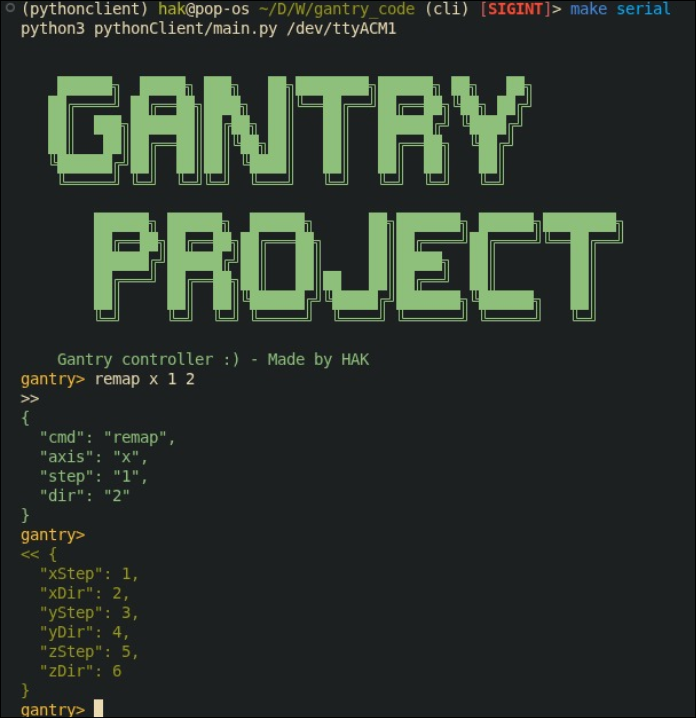
\includegraphics[width=1\linewidth]{gantry_project_cli.png}
    \caption{The Gantry CLI}
    \label{fig:gantry_cli}
\end{figure}